\subsection{Tipo de entidad Pregunta Asesor}

   \begin{description}

   \item[Definición] Se refiere al objeto del mundo real: \emph{``Cuestión
   perteneciente a una plantilla de entrevista de asesor planteada por el
   usuario asesor al usuario alumno''}.

   \item[Características] La entidad presenta las siguientes características:
      \begin{itemize}
         \item \textbf{Nombre:} Pregunta Asesor.
         \item \textbf{Tipo:} Débil por identificación con respecto a
         Plantilla Entrevista Asesor.
         \item \textbf{Número de atributos:} 3 propios y 3 heredados.
         \item \textbf{Atributo/s identificador/es principal/es:} id\_pregunta\_oficial.
         \item \textbf{Atributo/s identificador/es alternativo/s:} -
         \item \textbf{Atributo/s heredado/s:} dni\_pasaporte, curso\_académico
         además del atributo id\_entrevista\_asesor del tipo de entidad
         Plantilla Entrevista Asesor.
      \end{itemize}

   \item[Diagrama] La figura \ref{diagramaPregAse} muestra el diagrama de la entidad.
   \item \begin{figure}[!ht]
            \begin{center}
            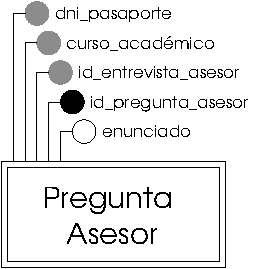
\includegraphics[]{07.Modelo_Entidad-Interrelacion/7.2.Analisis_Entidades/diagramas/preg_ase.pdf}
            \caption{Diagrama de la entidad Pregunta Asesor.}
            \label{diagramaPregAse}
            \end{center}
         \end{figure}

   \item[Descripción de los atributos propios] La entidad presenta los siguientes
   atributos propios:

   \begin{itemize}
    \item \textbf{id\_pregunta\_asesor}
      \begin{itemize}
         \item \textbf{Definición:} Código que sirve como número identificativo
               para cada pregunta de asesor del sistema.
         \item \textbf{Dominio:} Números naturales.
         \item \textbf{Carácter:} Obligatorio.
         \item \textbf{Ejemplo práctico:} 72.
         \item \textbf{Información adicional:} El dato lo genera el sistema
               cuando se introduce una nueva pregunta de asesor en el sistema.
               Es la clave primaria.
      \end{itemize}
   \item \textbf{enunciado}
      \begin{itemize}
         \item \textbf{Definición:} Cuestión perteneciente a una entrevista
         de asesor, planteada a un alumno.
         \item \textbf{Dominio:} Conjunto de caracteres alfanuméricos.
         \item \textbf{Carácter:} Obligatorio.
         \item \textbf{Ejemplo práctico:} Nivel de inglés.
         \item \textbf{Información adicional:} El dato lo introduce el
         usuario administrador al introducir una nueva pregunta de asesor en
         el sistema.
      \end{itemize}
    \item \textbf{última\_modificación}
      \begin{itemize}
         \item \textbf{Definición:} Establece el día, mes y año cuando se
            produjo la última modificación de la entidad.
         \item \textbf{Dominio:} Formato de fecha: dd/mm/aaaa.
         \item \textbf{Carácter:} Opcional.
         \item \textbf{Ejemplo práctico:} 02/02/2009.
         \item \textbf{Información adicional:} El dato lo genera el sistema
               cuando se modifica una pregunta de asesor en el sistema.
      \end{itemize}
   \end{itemize}

   \item[Ejemplo práctico]

   \item \begin{center}
            \begin{tabular}{ | l | l | }
            \hline
            \multicolumn{2}{ | c | }{\textbf{Tipo de entidad Pregunta Asesor}} \\
            \hline
            dni\_pasaporte & 98765432Z \\
            \hline
            curso\_académico & 2008 \\
            \hline
            id\_entrevista\_asesor & 36 \\
            \hline
            id\_pregunta\_asesor & 72 \\
            \hline
            enunciado & Nivel de inglés \\
            \hline
            última\_modificación & 02/02/2009 \\
            \hline
            \end{tabular}
         \end{center}
   \end{description}
